\documentclass[tikz,border=4pt]{standalone}
\usepackage{amsmath,amssymb}
\usetikzlibrary{arrows.meta,calc,decorations.pathreplacing}
\definecolor{cA}{HTML}{924800}
\definecolor{cB}{HTML}{2F7FC8}
\definecolor{cC}{HTML}{39994B}
\tikzset{
  pt/.style={circle,fill=black,inner sep=0pt,minimum size=4pt},
  disp/.style={-{Stealth[length=2.6mm,width=2mm]},line width=0.9pt,shorten <=2.5pt,shorten >=2.5pt},
  lab/.style={font=\small,sloped,text=black},
  brc/.style={decorate,decoration={brace,amplitude=5pt,raise=3pt},line width=0.6pt},
}
\begin{document}
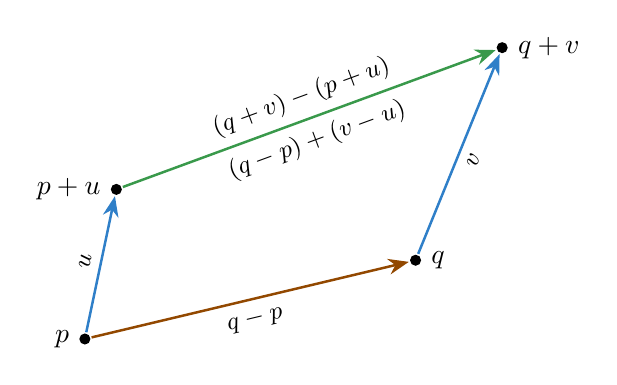
\begin{tikzpicture}
  \coordinate (p) at (0,0); \coordinate (q) at (4.2,1.0);
  \coordinate (pu) at (0.4,1.9); \coordinate (qv) at (5.3,3.7);
  \draw[disp,cA] (p) -- node[lab,below]{$q-p$} (q);
  \draw[disp,cB] (p) -- node[lab,above]{$u$} (pu);
  \draw[disp,cB] (q) -- node[lab,below]{$v$} (qv);
  \draw[disp,cC] (pu) -- node[lab,above]{$(q+v)-(p+u)$} node[lab,below]{$(q-p)+(v-u)$} (qv);
  \node[pt,label=left:$p$] at (p) {}; \node[pt,label=right:$q$] at (q) {};
  \node[pt,label=left:$p+u$] at (pu) {}; \node[pt,label=right:$q+v$] at (qv) {};
\end{tikzpicture}
\end{document}
